\chapter{Features}

\section{Namensgebung}
\begin{figure}[h]
  \centering
  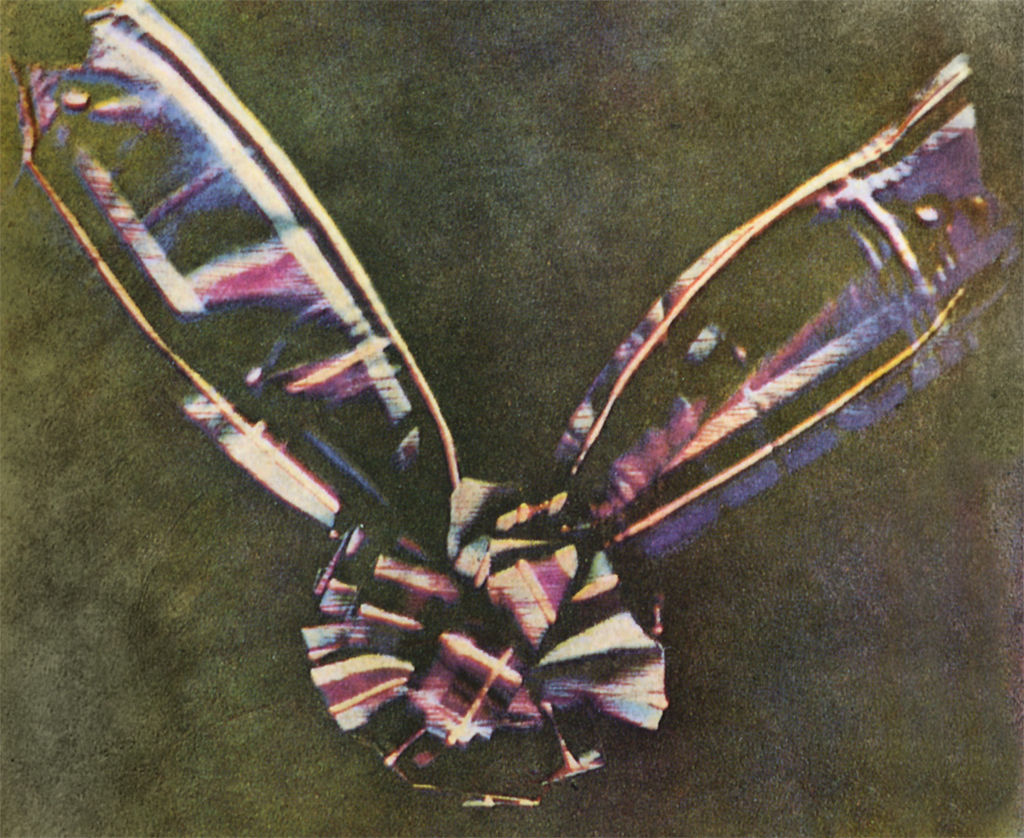
\includegraphics[width=0.7\textwidth]{images/tartan_band.jpg}
  \caption{Quelle: \url{Wikipedia.org}}
\end{figure}
Die erste bekannte Farbaufnahme war ein Tartan-Band.

\section{Anforderungen an Besucher}\label{besAnforderungen}
Browser ab folgender Version (theoretisch, getestet wurden nur Internet Explorer 11 und die zum Januar 2015 aktuellsten Versionen der restlichen bekannten Browser):
\begin{itemize}
	\item Chrome 10 (Release: 8.3.2011)
	\item Firefox 3.6 (Release: 21.1.2010)
	\item Internet Explorer 10 (Release: 4.9.2012)
	\item Opera 11.6 (Release: 6.12.2011)
	\item Safari 5.1 (Release: 21.7.2011)
\end{itemize}

Für manche Funktionen wird Javascript benötigt. Optimal sollte es daher für die Verwendung der Gallerie eingeschaltet sein.

\section{Voraussetzungen für den Webserver}
Auf dem Webserver müssen folgende Pakete instaliert sein
\begin{itemize}
	\item Python 3
	\item Django
	\item Pillow
\end{itemize}